% Chapter 3
\section*{Preface}
In this chapter we discuss the methods used when assembling a lab-scale battery for preliminary electrochemical tests. 
\pagebreak
\chapter{Experimental methods} % Main chapter title

\label{chap3} % For referencing the chapter elsewhere, use \ref{Chapter1} 

\section{Components of a cathode}
A cathode consists of an active material, a binder and conductive carbon. They are mixed together to form a slurry, which is then coated on a current collector.  
\begin{itemize}
    \item Active material: The main material that gives a battery its capacity
    \item Binder: A binder is usually a polymer that uniformly binds the cathode materials and allows it to stick firmly on the current collector. Polytetrafluoroethylene (PTFE or Teflon) and Polyvinylidene fluoride (PVDF) are most commonly used as binders while making battery slurries.
    \item Conductive carbon: A conductive form of carbon which is amorphous in nature, is added to improve the conductivity of the slurry. Super-P\textsuperscript{\textregistered} or carbon black is normally used as a conductive agent. 
    \item Current collector: Typically a metallic foil (copper, aluminium, steel, etc.) connected to the electrode with external loading. The main role of the current collector is to support the electrode and to collect the accumulated electrical energy from the electrode\cite{sun_effect_2017}.
\end{itemize}

\section{Formation of slurry}
A slurry is a paste-like substance used in making battery electrodes. It is important for slurries to be homogeneous. This helps in getting a uniform coating at later stages.  PVDF was mixed separately in an organic solvent, N-methyl pyrrolidinone (NMP). This viscous solution was added to the mixture of active material and Super-P\textsuperscript{\textregistered} . NMP can be added later to adjust the consistency of the slurry. It was then mixed on a magnetic stirrer for 8-10 hours. 

\section{Preparing a cathode}
Once the slurry was prepared, it was 'doctor-bladed' on a current collector. Doctor blading is a coating process where the slurry spreads on a substrate (molybdenum foil)  using a blade, to form a this sheet which dries off to give a layer of coating.  Initially, we used nickel foils as current collectors, however we found that Ni oxidised at $\sim$ 1.0 V. This did not allow the cell to reach it's cut-off potential at 2.4 V. It impeded the cell's redox processes, which reduced the cell's capacity. After trying a few current collectors, we found that molybdenum foil was inert in this cell chemistry (discussed in Appendix A) and was used in all our battery systems. After coating the foils with the slurry, the electrodes were dried at 80$^{\circ}$ C for two hours to improve the adhesion of the slurry onto molybdenum foil. 

\begin{figure}[tbh!]
\centering
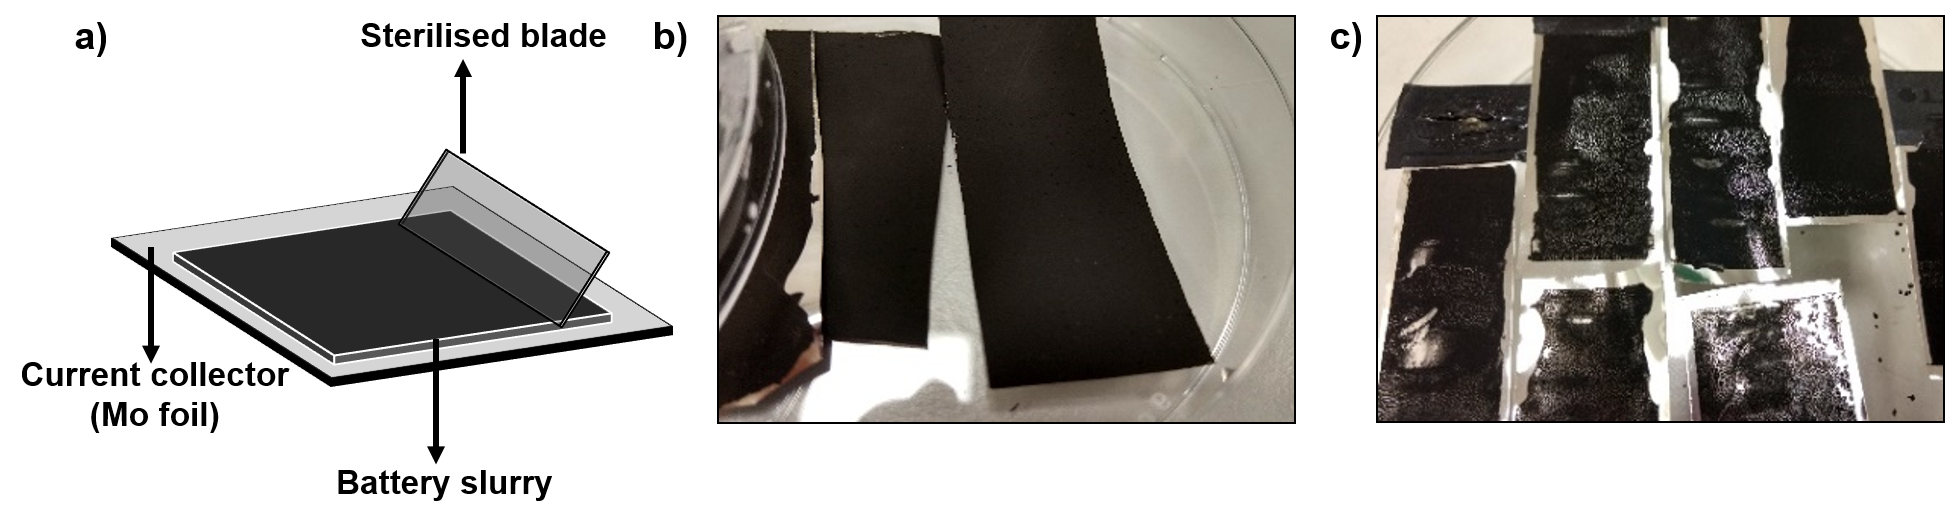
\includegraphics[width=\textwidth]{Figures/chap3fig/coating}
\caption{a) Doctor-blading on a current foil using a steel blade. A dried cathode after b) uniform and c) non-uniform coating.}
\label{Figures/chap3fig:coating}
\end{figure}

\section{Vacuum drying}
Vacuum drying is a moisture-removal technique by means of creating a vacuum. Vacuum drying is used for drying things which are hygroscopic (water sensitive). IA vacuum is created to decrease the chamber pressure below vapor pressure of the solvent (NMP), causing it to boil. This increases its rate of evaporation and increases the drying rate of the product. The pressure maintained in vacuum drying is generally 0.03-0.06 atm. The cathodes are ready for use after drying. 

\section{Assembling a cell}
Using pouch cells or coin cells (CR-2032\textregistered) is a common practice amongst researchers working on batteries. CR-2032 is made of steel and could not be used in our experiments. Since our electrolyte reacts with steel, we switched to custom-made cells that used PEEK (polyether ether ketone) for the main body and steel rods as plungers that would push the electrodes towards each other. PEEK  is a colourless organic thermoplastic polymer. It has a melting point of 343$^{\circ}$C, with excellent mechanical and chemical resistance properties. Steel rods were later replaced with molybdenum rods because of above mentioned reasons. 

\begin{figure}[tbh!]
\centering
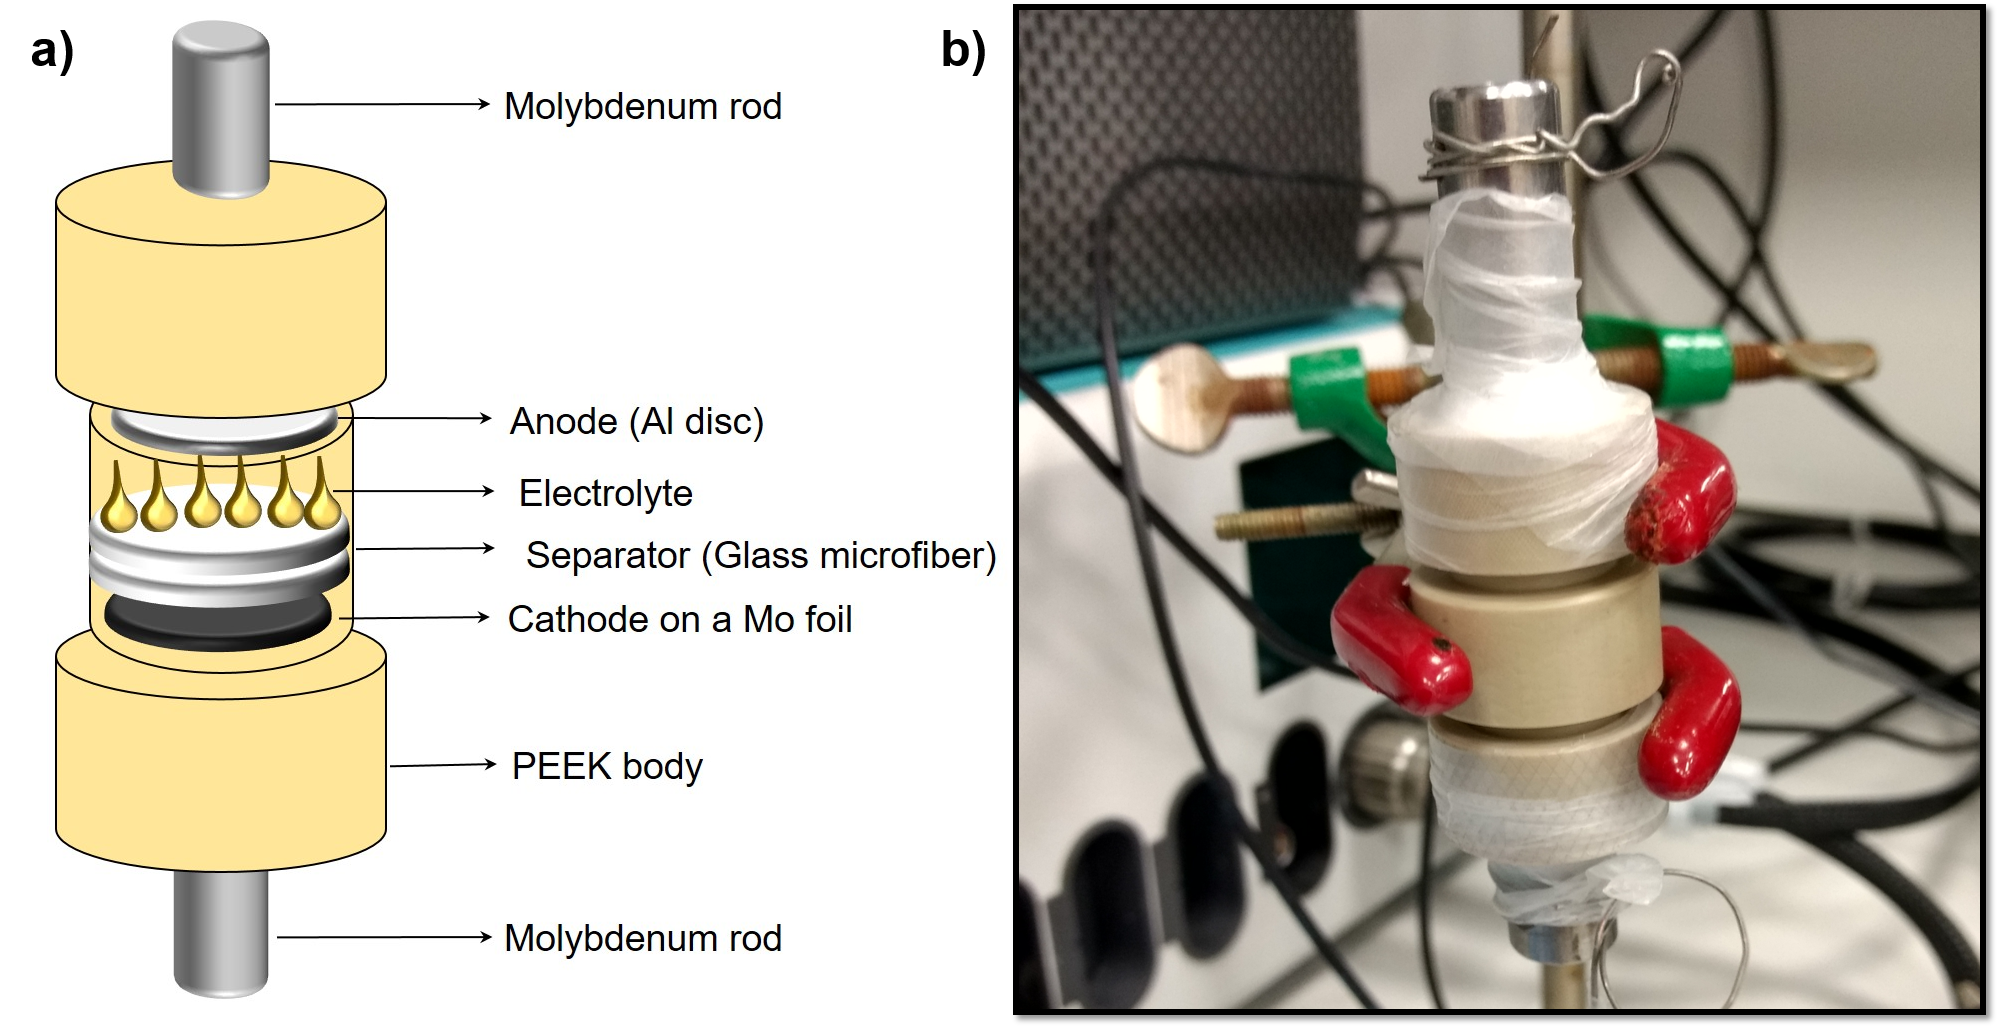
\includegraphics[width=\textwidth]{Figures/chap3fig/swagelok}
\caption{a) Assembling a two-electrode PEEK cell using a cathode, separators wetted with electrolyte and an anode. Mo rods were used as plungers and Mo sheets was used as current collector. b) A custom-made lab cell ready for preliminary electrochemical measurements.}
\label{Figures/chap3fig:swagelok}
\end{figure}

A cathode was placed at the bottom of the cell, two separators made of glass microfibers were put above the cathode. Electrolyte was then added ($\sim$80 $\mu$l) until the separators were completely wet. An anode which was 99\% pure aluminium foil was cut into a disc and placed on top and the cell was then screwed tight, shown in Figure \ref{Figures/chap3fig:swagelok}a. Since the electrolyte is hygroscopic, the cell was assembled inside a glove box with <0.1ppm \ce{O2}, \ce{H2O}. The cell was taken out of the glove box and wrapped tightly with a paraffin film to further inhibit contact with moisture or air, as shown in Figure \ref{Figures/chap3fig:swagelok}b. The cell was then ready for electrochemical measurements . 





















